\documentclass{article}

% Uncomment for the camera-ready ``final'' version
%\usepackage{corl_2019} % initial submission
\usepackage[final]{corl_2019} 
\usepackage{amsmath}
\usepackage{graphicx}
\usepackage{wrapfig}
\usepackage{natbib}

\title{Interactive Segmentation using Object Singulation}

% NOTE: authors will be visible only in the camera-ready (ie, when using the option 'final'). For the initial submission the authors will be anonymized.

\author{
    Patrick Pfreundschuh\\
    Autonomous Systems Lab\\
    ETH Zuerich \\
    \texttt{patripfr@ethz.ch} \\
    \And
    Simon Schaefer \\
    Autonomous Systems Lab\\
    ETH Zuerich \\
    \texttt{sischaef@ethz.ch} \\
    \AND
    \Coauthor \\
    Michel Breyer \\
    Autonomous Systems Lab\\
    ETH Zuerich \\
    \And
    \Coauthor \\
    Fadri Furrer \\
    Autonomous Systems Lab\\
    ETH Zuerich \\
    \And
    \Coauthor \\
    Tonci Novkovic \\
    Autonomous Systems Lab\\
    ETH Zuerich \\
}

\newcommand{\myeqref}[1]{Eq.~\ref{#1}}
\newcommand{\myfigref}[1]{Fig.~\ref{#1}}
\newcommand{\mysecref}[1]{Section~\ref{#1}}
\newcommand{\mytableref}[1]{Table~\ref{#1}}

\begin{document}
\maketitle

%===============================================================================

\begin{abstract}
An accurate segmentation is crucial for performing manipulation tasks in real-world environments, but especially in cluttered environments is still poses a problem as adjacent objects are segmented together. This problem can be solved by enhancing visual with interactive segmentation, using push movements to singulate objects from each other. Current learning based approaches for this task use Deep Q-Learning (DQL) with a discretized action space. As using continuous actions instead would allow more complex and more efficient pushing movements, in this paper it was evaluated whether Proximal Policy Optimization (PPO) can also solve the task of object singulation. It is shown that with PPO only simple static scenes can be solved with the proposed setup, while in contrast also simple dynamic scenes could be solved using DQL.  
\end{abstract}

% Two or three meaningful keywords should be added here
\keywords{CORL, Robots, Learning}

%===============================================================================

\section{Introduction}
Detection of objects is of high importance for applications where robots are supposed to interact with the environment. Often robots are used to sort or arrange objects like in several household tasks or in general in pick and place tasks. To do so successfully, in most cases visual segmentation is used, which works already well for structured environments, where the objects can be easily identified.
However, handling unstructured environments that have to be manipulated is a major challenge in robotics, since often objects can only be viewed partially due to occlusion, which makes segmentation hard and thus complicates grasping of objects.
\newline
In order to simplify segmentation and picking under these conditions objects can be segmented interactively, e.g. the objects can be singulated, using push movements. However, efficient and precise object singulation still poses a problem, especially as a-priori the number of objects is unknown. Therefore, the robot has to explore, if a segmented area really consists of a single object, or if it might be multiple objects side by side. Furthermore, in applications where the robot should interact with objects that were unseen before, interactive segmentation can help to reason about the new and unknown object.
\newline
While previous approaches tackle the problem of object singulation by discretizing the state space, only allowing a limited number of actions, within this project we want to explore the feasibility of a continuous approach for object singulation. 

The main contributions of this paper are:
\begin{itemize}
\item A new reinforcement learning task design for continuous object singulation
\item Object singulation for a simple static task using a continuous policy
\item Object singulation for simple dynamic tasks using Deep Q-Learning
\item Illustration of pitfalls using unimodal policies
for object singulation tasks
\end{itemize}
%===============================================================================

\section{Related Work}
\label{sec:rel-work}
The problem of singulating objects can be tackled in various different ways in terms of manipulation techniques and policies. While some approaches use a robotic hand that only pushes objects in a two-dimensional manner \citep{guided_pushing}, others also use grasping for singulation \citep{interactive_singulation}. Clearly, grasping can facilitate the task, especially when it comes to objects that were segmented such that the agent is not sure whether it is a single or multiple objects. In the case of multiple objects side by side, the robot will with high chance only grasp one of the objects, while the other one remains unchanged. With pure pushing of objects, the appearance of multiple objects side by side might remain unchanged, depending on the direction they are pushed to. Hence, both the starting position as well as the pushing sequence itself are crucial for the success of the overall action, while for grasping dominantly the choice of starting point is important. However, physically executing a pushing action is a lot more straightforward and extendable to a bunch of different actuators compared to grasping. Therefore, allowing pushing actions only is a broad research area. 
\newline
Work can furthermore be split into approaches using hand-tuned deterministic policies or learning based approaches. \citeauthor{drl_synergies} et al. \citep{drl_synergies} have already successfully shown, that deep neural networks are capable of learning the discussed task using grasping and pushing, using two large 121-DenseNets in parallel, one predicting the Q values for pushing and one for grasping state-action-pairs. \citeauthor{push_proposal} et al. \citep{push_proposal} also showed that a network can learn to solve the problem using pushing only, by training a convolutional neural network which ranks certain pushing action by their priority. However, both approaches discretize the action space and use DQL, limiting the range of possible actions. To the best of our knowledge we are the first ones combining deep reinforcement learning with a continuous, pushing-only action space for the object singulation task. 
\newline
There are several deep reinforcement learning algorithms with continuous action space, such as off-policy and Q-value based methods as Deep Deterministic Policy Gradient \cite{ddpg} or on-policy advantage-based methods such as TRPO \cite{trpo}, A3C \cite{a3c} or PPO \cite{ppo}, whereby on-policy methods usually are more sample-efficient. While \citeauthor{drlthatmatters} et al. \cite{drlthatmatters} state Trust-Region-Policy-Optimization (TRPO) and PPO to be the most stable model-free policy gradient methods (i.e. having the smallest confidence bounds in reproduction) \citeauthor{baselines} et al. \cite{baselines} show that PPO outperforms TRPO in most common testing environments such as HalfCheetah, Walker2d and InvertedDoublePendulum and is easier to tune because of having less tuning parameters. PPO maximizes a surrogate advantage, estimated as $E[min(\rho_t(\theta) A_t, clip(\rho_t(\theta), 1 - \epsilon, 1 + \epsilon)A_t]$ which $A_t = R_t - V(s_t)$ being the advantage function and $\rho_t(\theta) = \pi(a_t | s_t, \theta) / \pi(a_t | s_t, \theta_{old}$ is the likelihood ratio of the action at timestep $t$ between the updated and sampled policies, clipped using the  hyperparameter $\epsilon$. 

%===============================================================================

\section{Method}
\label{sec:method}
In this project, a manipulator should learn to singulate objects using push movements only.  An RGD-D camera is used to perceive the environment. During this project, training was performed in a simulation which is further described in \mysecref{sec:simulation}. The infinite set of possible states, continuous actions as well as hardly predictable state transitions exacerbate deterministic modeling. Therefore a reward-based learning approach is used. Since a continuous policy was desired, PPO \citep{ppo} was chosen as reinforcement learning algorithm, as it has shown to be very successful for tasks, is easy to tune and a hence a favorable tradeoff between sample-complexity, simplicity, and wall-time as described in \mysecref{sec:rel-work}, combined with a deep fully connected network.

\subsection{Image Preprocessing}
\label{images}
Images are taken in a bird-eye view from above the object plane, since this minimizes occlusion. The depth channel of the RGB-D image is used to remove background from the objects, since only pixels with objects incorporate relevant information.
A 64x64 px binary mask is then created, indicating where objects are located. From the binary mask, a distance map is calculated. This map shows the distance (in pixel) to the closest object for each pixel. Pixels inside objects are set to $-1$. 

\begin{figure}[!ht]
\centering

\includegraphics[width=14cm]{figures/observations.png}
\caption{Different representations for a scenario where 3 quadratic blocks are placed next to each other. From left to right: RGB image observation, binary mask, distance map
}
\label{fig:observations}
\end{figure}

\subsection{Task}
Since the experiment scenarios used in this project can be solved with one push, one episode consists of one step, where one step corresponds to one push movement. The push movement is realized with a simulated gripper that performs a straight line motion, which is explained in more detail in \mysecref{sec:simulation}. 

The action space is heavily biased on non-successful actions, not touching any object. Choosing a starting point close to an object leads to a successful pushing action with higher probability than far from the object.  Therefore the learning task was implemented with the goal to lead the agent to choose actions close to objects

\subsubsection{State}
As input state, the 64x64 px distance map described in \myfigref{images} is used. This way, possible good starting points are already indicated by low distance values in the input map and good pushing directions can be obtained following the distance gradient at every position of the map. 

\subsubsection{Action}
The action consists of a point in the workspace and one of the four cardinal directions. The agent then performs a straight line push from this point in the chosen direction. A fixed length of one quarter of the workspace was chosen to reduce the complexity. \\
 Action $ a = (x,y,c)$ with $x,y  \in [-l,l] , c \in \{up,down,left,right\}$ where $l$ corresponds to half of the length of the workspace.

\subsubsection{Reward}
Since we want to singulate the objects from each other, a metric to maximize is the inter-object distance $d_{IO}$. The inter-object distance is defined as 
\begin{align}
d_{IO} = \sum_{i,j\in C }^{} d_{i,j}
\end{align}
   
where $C$ is the set of all combinations of two objects, i.e $C = {O_{seg}\choose 2}$ with $O_{seg}$ being the set of all segmented objects and $d_{i,j}$ is the distance between object $i$ and $j$.
Since the objects only have to be separated from each other by a fixed distance threshold $d_{goal}$, we are using the truncated inter-object distance $d_{IOT}$ defined as: 

\begin{align}
d_{IOT} &= \sum_{i,j\in C }^{} min(d_{i,j},d_{goal}) \\ 
r_{Dist_t} &= d_{IOT_{t}}-d_{IOT_{t-1}}
\end{align}

This way, the agent receives a reward if the truncated inter-object distance is increased, and is punished if it is decreased. If two objects that were segmented as one before become singulated, this will result in new summands in $d_{IOT_t}$ since $O_{seg_t}$ will be bigger than $O_{seg_{t-1}}$.
\newline
To set an incentive to start close to objects, a second reward $r_{Start}$ is added. Starting far away very often results in a non-rewarding pushing, as no object is hit. At the same time, starting very close to an object might be not feasible having a real-world robot gripper in mind. Therefore, $r_{Start}$ is defined peaking at a goal distance ($d_{Goal}=0.2 m$), while decreasing when moving closer to the object as well as further away from the goal distance:

\begin{align}
r_{Start}(d_{Object}) = \begin{cases} 
K_1*sigmoid(d_{Object}) + K_2 & \text{if } d_{Object} \leq d_{Goal} \\
K_3/d_{Object} + K_4 & \text{otherwise}
\end{cases}
\end{align}

Additionally, a penalty $r_{Inside}$ is given, if a starting point inside an object is chosen (since this action can not be applied in a real world). Furthermore, if objects are separated successfully, a fixed success reward is added. 

\begin{minipage}[b]{0.49\textwidth}
\begin{align}
r_{Inside} = \begin{cases}
1 & (x,y) \text{ is in object} \\
0 & \text{else}
\end{cases}
\end{align}
\end{minipage}
\begin{minipage}[b]{0.49\textwidth}
\begin{align}
r_{success} = \begin{cases}
1 & d_{IO}\geq d_{IO_{goal}} \\
0 & d_{IO}< d_{IO_{goal}} 
\end{cases}
\end{align}
\end{minipage}

The total reward is then calculated as shown in \myeqref{eq:reward_all}. For our experiments we chose $k_{Start}=300$, $k_{Dist}=1000$, $k_{Inside}=-100$, $k_{Success}=1000$. This way, a very high reward is given for successful singulation, a high reward is given for partial singulation, a small reward is given for choosing a close starting point and a small penalty is given for starting inside an object.

\begin{equation}
r_t = r_{Start}*k_{Start} + r_{Dist}*k_{Dist} + r_{Inside}*k_{Inside} + r_{Success}*k_{Success} 
\label{eq:reward_all}
\end{equation}

\begin{figure}[!ht]
\centering
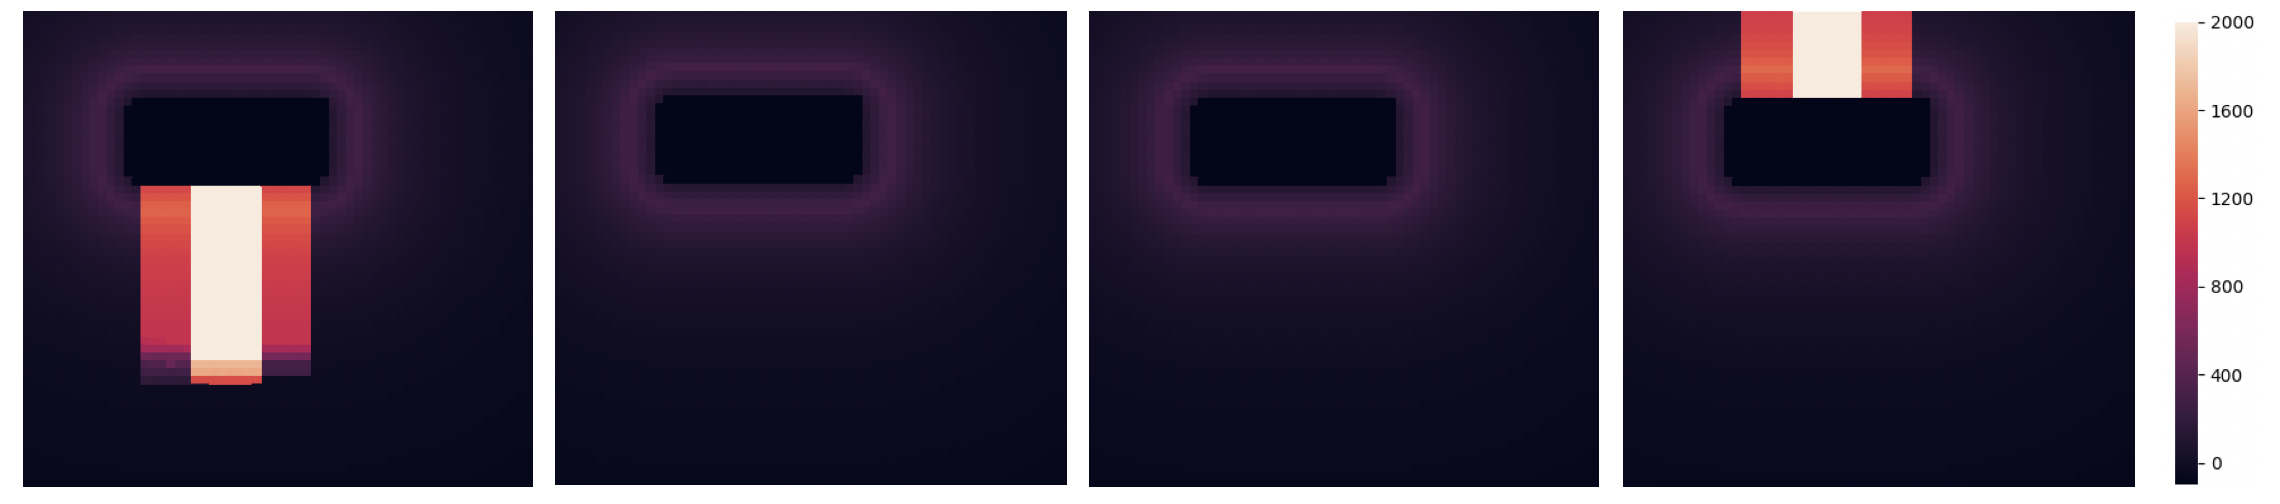
\includegraphics[width=14cm]{figures/rewards.png}
\caption{Reward heatmaps for all cardinal pushing directions for scenario shown in \myfigref{fig:observations}, 
mapped by starting point (from left to right: up, right, left, down)
}
\label{fig:rewards}
\end{figure}

\subsection{Network Architecture}
The network used for the results consists of 5 fully connected layers with units [128,64,64,32,16] and ReLU activation after each layer. During the design of the network, it has shown that smaller networks than the proposed could not model the task's complexity.
%===============================================================================

\section{Simulation Setup}
\label{sec:simulation}
For simulation the pybullet simulation engine\footnote{https://pybullet.org} was used, enabling basic rigid body physics, with the goal to model an interactive object singulation task close to a real-world application. The objects are therefore placed on a table with finite dimensions and observed by a fixed RGBD camera on top of it. The objects that are to be segmented are cubic, oriented in parallel to the table, varying in size and either always placed at the same position repeatedly (\textit{fixed scenario}) or placed randomly (\textit{random scenario}). The actuator is modelled as a small block being able to start anywhere in the scene, position controlled and having a comparably large mass in order to ensure that the determined action is executed as stated. Modeling the scene using simple cubes thereby reduces the problem to a fundamental level and speeds up the training procedure, since a comparably computationally efficient simulation configuration, i.e. a comparably high time step ($= 0.01 s$) and low number of solver iterations ($= 100$), can be used. Before and after executing an action, the camera takes an image (64x64x3), which serves as input for the learning agent as well as for determining the reward, after being pre-processed as described in \mysecref{sec:method}. The depth channel is thereby used to determine which pixels correspond to objects and which to the background. In order to represent the real-world scenario as good as possible no further data from the simulation is used for the proposed algorithm. 

%===============================================================================
\section{Experimental Results}
\label{sec:result}

Since there are no established baselines for a continuous approach to solve object singulation, an approach that was used in the beginning of the project is used to show how the task defined in \mysecref{sec:method} improved learning efficiency. This earlier approach uses simpler representations for state, action and reward. In detail, the following is compared: \\
The state representation of our approach is compared to a simple binary map. This binary map indicates if a pixel belongs to an object or background.
The reward of our approach is compared to another reward using only a difference of inter-object distance reward, i.e. $r_t=r_{Dist_t}$. Finally, we compare the reduced action definition proposed in our approach with a more basic action definition that simply predicts the start and end point of the pushing line, i.e  $ a = (x_{Start},y_{Start},x_{End},x_{End})$ with $ x_{Start},y_{Start},x_{End},x_{End}  \in [-l,l]$.

\subsection{Experimental Setup}
As a reinforcement learning framework we used the Baselines framework from OpenAI \citep{baselines}. 
The following parameters were used for PPO training:
\begin{table}[!htbp]
\centering
\label{tab:tuning_param}
\begin{tabular}{|l|c|c|c|}

\hline 
\textbf{Configuration parameter} & \textbf{Value}  \\ \hline
Learning rate	 		& $5e-4$	  \\ \hline
Mini-Batchsize	 		& $4$	 	   \\ \hline
Batch size	 & $2048$	    \\ \hline
Number of Training epochs per update	 & $3$	    \\ \hline
\end{tabular}
\caption{PPO configuration}
\end{table}

\subsection{Improvement of Learning Efficiency}

\begin{wrapfigure}[25]{r}{5.5cm}
\centering
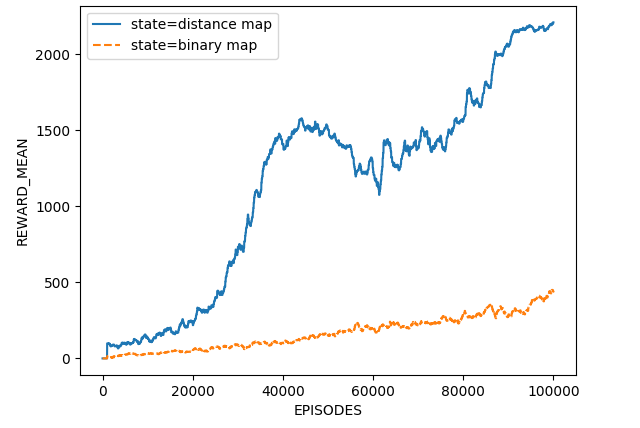
\includegraphics[width=5.5cm]{figures/efficiency-state.png}
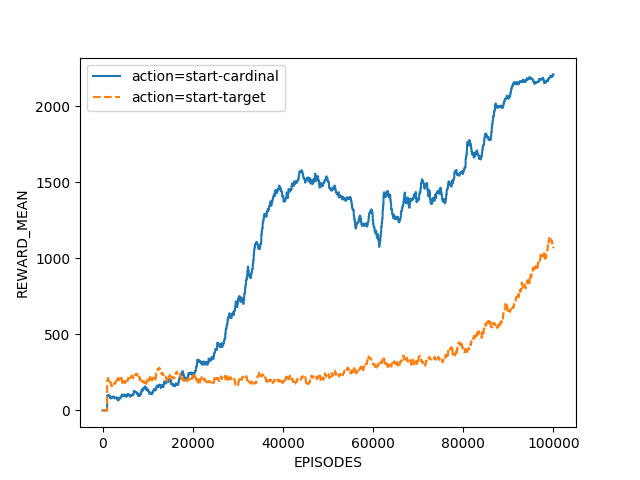
\includegraphics[width=5.5cm]{figures/efficiency-actions.png}
\caption{Learning sample-efficiency improvements of the proposed against the baseline task (1: state, 2: action}
\label{fig:efficiency}
\end{wrapfigure}

In the following the impact of the proposed approach is compared to the baseline approach defined above, for a scenario where two connected blocks are always positioned at the same points. \myfigref{fig:efficiency} displays a direct comparison between them in terms of their convergence of the reward between the state, action and reward definition (blue: proposed approach, orange: baseline approach).  
\newline
As described in \mysecref{sec:method} the distance map introduces a bias for good starting point choices, compared to a binary map, which does not differ between pixels close and far away from an object. Consequently, as shown in \myfigref{fig:efficiency} a model trained on the distance map converges much faster. The reward as specified in \mysecref{sec:method} is only large, if blocks are separated from each other, touching the blocks while not separating them does not return any ($r_{Dist}$) reward. Using a starting point and cardinal direction only instead of predicting both the start and end position of the action reduces the number of possible actions but increases the ratio between succeeding and failing actions, since, although there are less possible starting position from which an object can be hit, the cardinal pushing direction (applied on the cubes we use as objects in simulation) guarantees separating the objects as good as possible, whereas the start-target-action might lead to hitting but not separating objects. 

\begin{wrapfigure}[27]{r}{5.5cm}
\centering
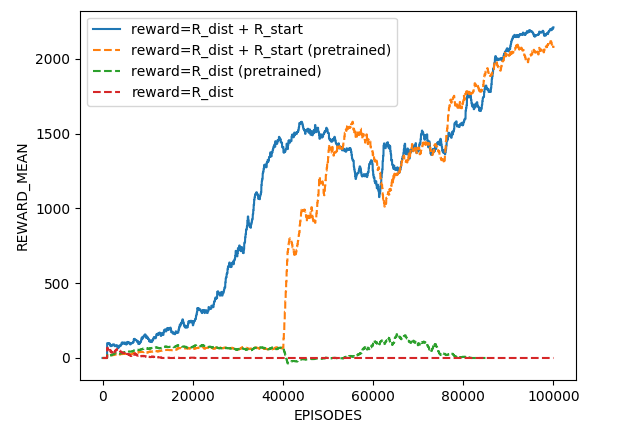
\includegraphics[width=5.5cm]{figures/efficiency-reward.png}
\caption{Learning sample-efficiency improvements of the proposed against the baseline task for reward definition} 
\label{fig:rdiffdist}
%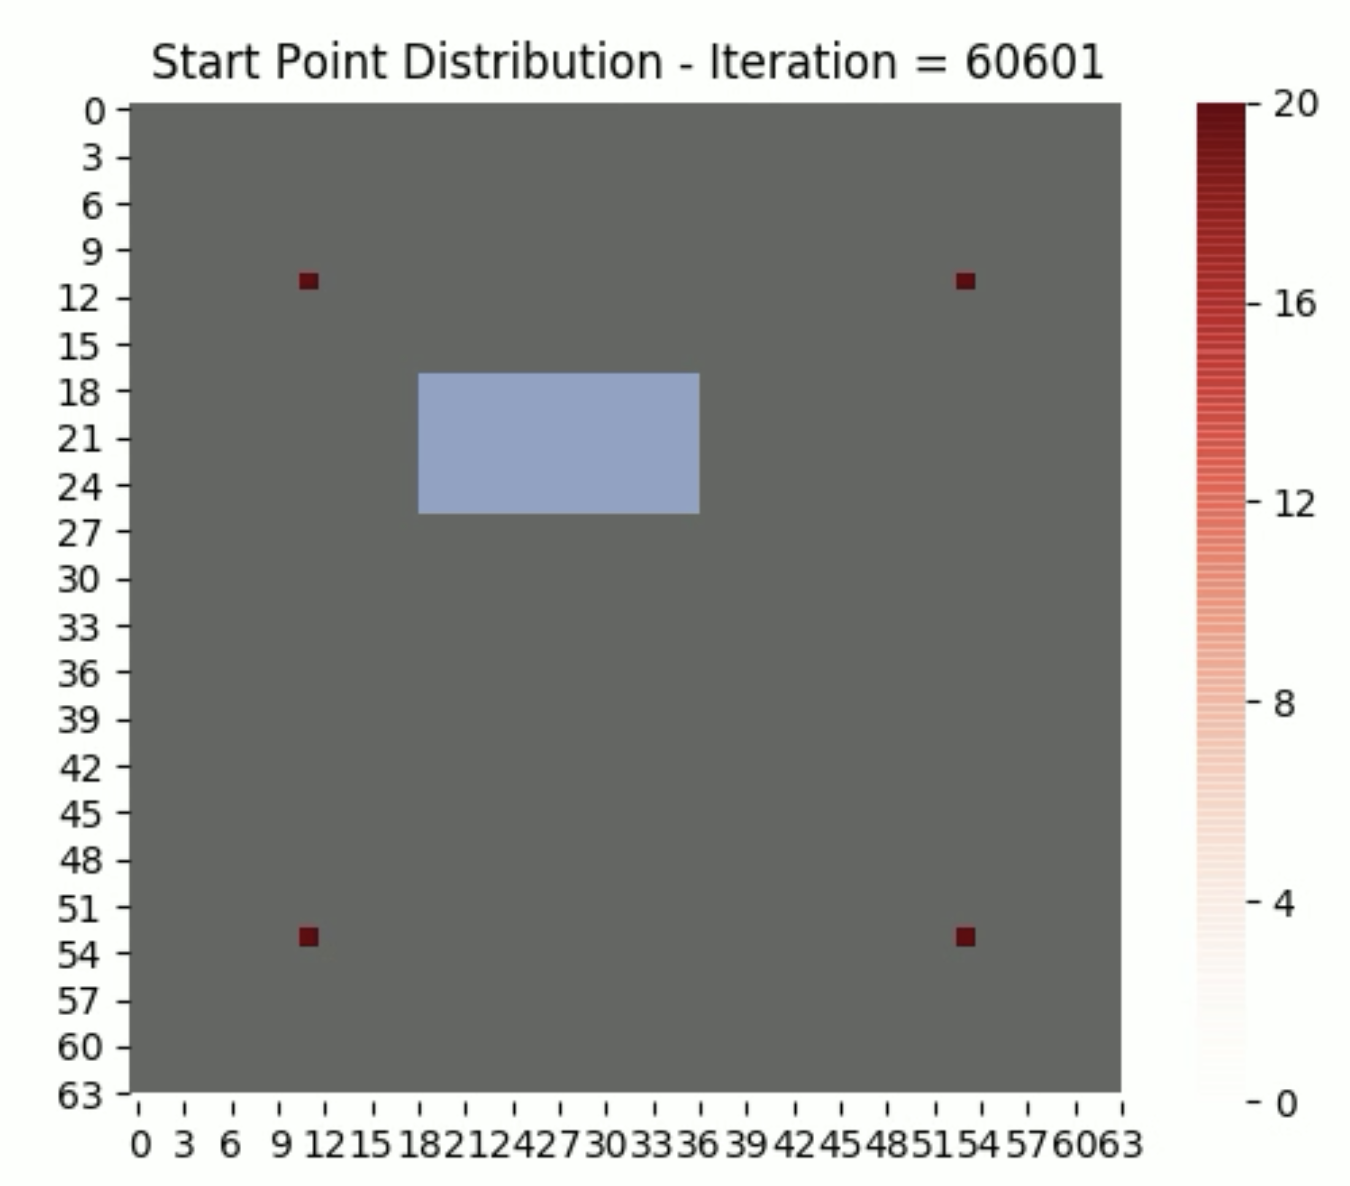
\includegraphics[width=5.5cm]{figures/rdiffdist-actiondist.png}
%\caption{Final action start position frequency for scenario $r = r_{Dist}$}
%\label{fig:actiondist}
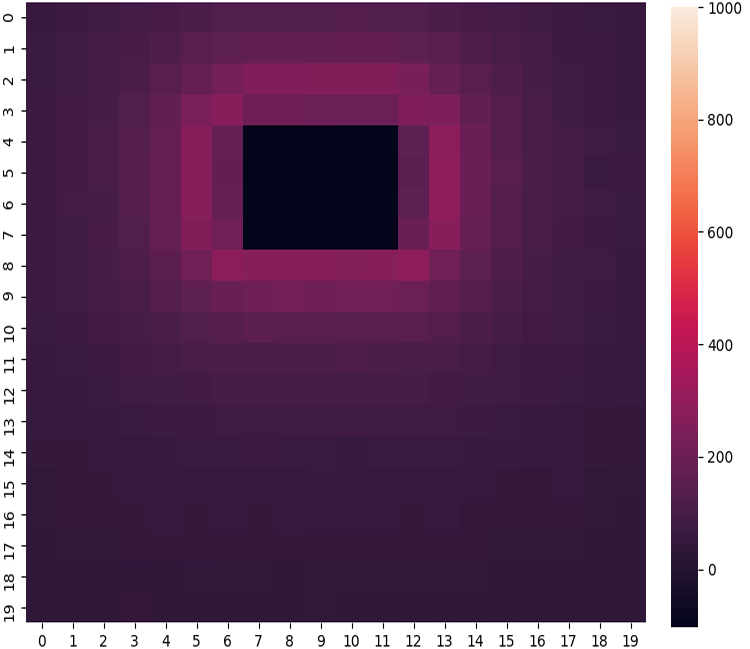
\includegraphics[width=5.5cm]{figures/q_values_quad.png}
\caption{Q-Values for the task explained in \mysecref{sec:unimodality} after 4000 steps.}
\label{fig:qvalues}
\end{wrapfigure}

\myfigref{fig:rdiffdist} compares the evolution of the returned reward for several reward function definitions. In this context \textit{pretrained} refers to a scheduled reward function, returning $r = r_{Start}*k_{Start} + r_{Inside}*k_{Inside}$ only in the first $40*10^3$ iterations. As explained in \mysecref{sec:unimodality} merely rewarding a successful pushing movement is too sparse to guide to a good policy. Pretraining can improve the sparsity of the reward by introducing a bias to the starting position to be close to an object and can therefore slightly improve the result, however using $r_{Start}$ for all training iterations is necessary to come up with a highly-valued policy, as shown in \myfigref{fig:rdiffdist}($r = R_{Dist} + R_{Start} (pretrained)$). 

\subsection{PPO Unimodality Issue}
\label{sec:unimodality}
While a simple fixed scenario with two blocks could be solved using PPO, it failed when it came to scenarios, where blocks are positioned at random positions. We believe that the reason for this lies in the unimodality of the gaussian probability density funtion used in the PPO implementation.
In general object singulation tasks, the reward usually is multimodal. This is due to the fact, that the problem has multiple symmetries in most cases. E.g. in the scenario shown in \myfigref{fig:ppo_evolution} the agent will receive the same reward if it starts on top of the object and pushes downwards or if it starts below the object and pushes upwards. At the same time, all starting points in between (i.e. points inside the object) will lead to a negative reward, since starting inside the object is not possible. However PPO uses unimodal gaussian policies to capture the reward \citep{ppo}\citep{Tang2018}. 
\newline
To visualize this behaviour the agent was trained to only spawn close to the object ($r = r_{Start}*k_{Start} + r_{Inside}*k_{Inside}$). As seen in \myfigref{fig:ppo_evolution} PPO first tries to capture this multimodal distribution with a unimodal policy with high variance and mean inside the block, which complicates converging to one highly rewarded action.

% The PPO agent behaves similarly,  in the scenario 
% $r = r_{Dist}$ converging to zero reward as displayed in \myfigref{fig:rdiffdist}. Beginning to place the action's start position randomly, the agent keeps increasing the variance of the unimodal policy distribution. In order to perform an action in the simulation the action has to be in $[-l,l]$, applying an activation function (like e.g. $tanh$) in order to map the agent's output to $[-l,l]$ however complicates converging to a good starting position since the transformation between block and good start position depends on the block's position (non-linearity). Therefore, the action is clipped to $[-l,l]$. An increasing variance of the policy distribution then leads to sampling values at the edge of the allowed action space, which do not lead to a reward, which again leads to increasing variance. 

In a scenario where blocks are placed randomly and also including push directions, this behaviour becomes even more problematic, such that for our object singulation task PPO was not able to solve random scenarios.

\begin{figure}[!ht]
\centering
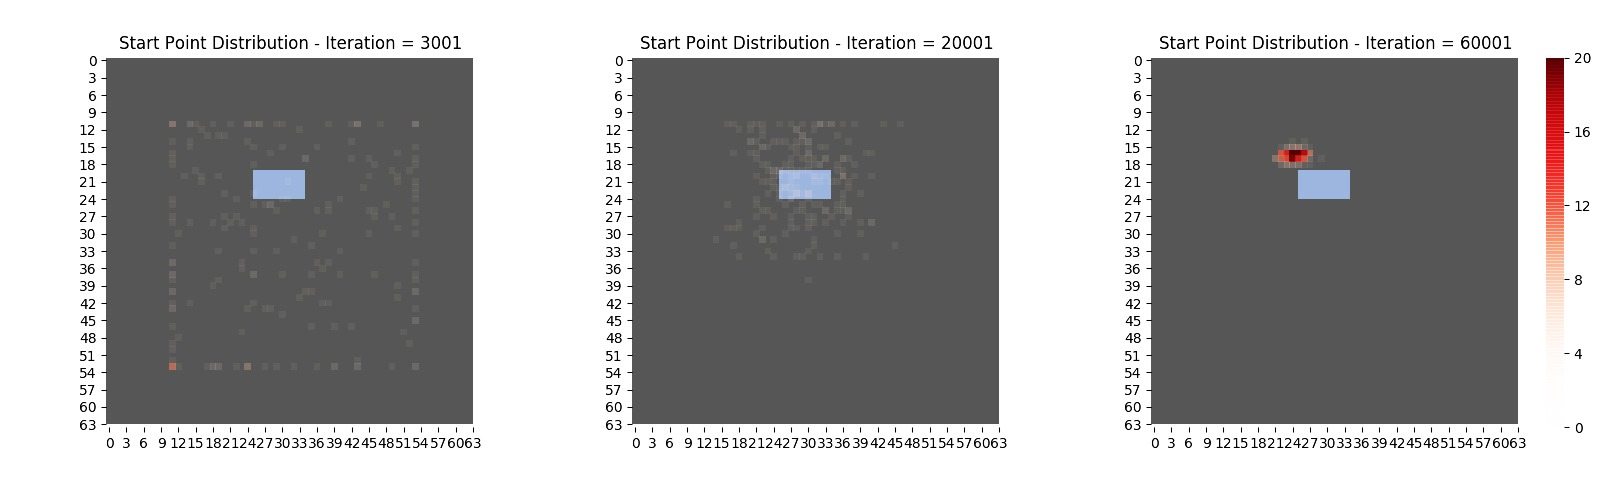
\includegraphics[width=14cm]{figures/ppo_distribution_evolution.jpeg}
\caption{Action start position frequency evolution over 60000 iterations. It can be seen, that the Gaussian is centered at the object after 20000 iterations, while it takes additional 40000 iterations to converge to one specific spot.}
\label{fig:ppo_evolution}
\end{figure}

\subsection{Deep Q-Learning Results}
To show, that the task is learnable with the proposed setup, we also applied Deep Q-Learning \citep{deepq}. The same network, state, and rewards as described in \mysecref{sec:method} were used, while the action's start point had to be discretized in order to make it compatible with Deep Q-Learning. We discretize the workspace in 10 segments in both directions of the plane. This allowed us to solve simple scenarios where 2 or 3 blocks where placed connected at random positions. Videos of those results can be found at \href{https://bit.ly/2EYsDJ4}{https://bit.ly/2EYsDJ4}. 
\newline
%However, this was only used as a proof of concept in the last weeks of the project. More complex scenarios that can only be solved in multiple steps were not solved yet. 
It could also be shown that Deep Q-Learning converged much faster for the task that was used in \myfigref{fig:ppo_evolution}. As shown in the Q-Value visualization below, the Q-Values already converged to a correct representation after $4000$ steps, while it took PPO $60000$ steps to converge to one point. Next to better performance for the proposed task, DQL is also capable of finding optimal policies in cases in which PPO fails, e.g. the $r = r_{Dist}$ scene. Due to the random exploration, DQL is less likely to get stuck in a cyclic behaviour especially in the beginning of the training. Thus, DQL can find a good policy for the $r = r_{Dist}$ scenario. 

%===============================================================================

\section{Conclusion}
\label{sec:conclusion}
Within this project the feasibility of applying more continuous, experience-based approaches, specifically PPO, for the object singulation task was examined. Although improvements in terms of sample-efficiency of PPO were made, it was shown that it is merely applicable to simple and fixed scenarios, as it is not able to model multimodal policies, while random scenarios could be solved using DQL.
\newline
We have shown that using PPO is not a feasible approach for solving the object singulation task as we defined it, our insights are however transferable to other continuous (advantage-based) reinforcement learning algorithms like TRPO \citep{trpo}, that also use unimodal policy distributions. In future work in order to use a continuous action space in an object singulation task either an approach with a multimodal policy space could be used or the transformation of the task from a multimodel to a unimodal definition could be learned, e.g. by using Fourier transformation parametrizing the multimodality. For learning efficiency of both a continuous and a discrete action the state-space could be downsized to a more dense representation using an autoencoder. While the project focused on simulation only, further work could also apply the proposed method to a real-world scenario, such as a pre-segmentation step.   

%===============================================================================

% The maximum paper length is 8 pages excluding references and acknowledgements, and 10 pages including references and acknowledgements

\clearpage
% The acknowledgments are automatically included only in the final version of the paper.

\acknowledgments{
We would like to thank a number of people who have encouraged and helped us in realizing this Semester Project. We appreciate the support we received from all sides.
\vspace{0.5cm}
\newline
We want to thank Prof. Dr. Roland Siegwart for offering this course, and the possibility to do a project in this format.
\vspace{0.5cm}
\newline
We also appreciate the feedback about the proposal and intermediate report from Dr. Cesar Cadena and Dr. Jen Jen Chung, who also made this project possible at all by allowing us to create a reinforcement learning project together with our supervisors.
\vspace{0.5cm}
\newline
Special thanks to our supervisors Fadri Furrer, Tonci Novkovic and Michel Breyer. Their broad knowledge and experiences in reinforcement learning had a wide influence on the results.
\vspace{0.5cm}
\newline
Zurich in June 2019,
\newline
Simon Schaefer \& Patrick Pfreundschuh
}

%===============================================================================

% no \bibliographystyle is required, since the corl style is automatically used.
\bibliography{example}  % .bib

\end{document}
